\chapter[ADC on AVR based microcontroller]{Analog to Digital Conversion in AVR microcontroller}
In this chapter we will study the working of the Analog to Digital Conversion in AVR microcontroller.
\section{What is ADC?}
For reactive embedded system, digital microcontroller system has to interact with the external environment such as temperature, humidity, speed and many more. For sensing these external environment we use sensors which gives output in form of analog voltages. So for bridging the gap between analog voltages into digital equivalent AVR microcontrllers has internal 10-bit ADC.
After getting digital value from ADC we can use them in the code.

Sensors and signal conditioning are large topics which will not be discussed in this chapter. But we will focus on operation of ADC present in AVR based microcontroller and study how to operate the ADC.
\section{Major Blocks of ADC}
ADC is one of the independent block present in AVR microcontroller. It consists of blocks as shown in Figure \ref{fig:ADC}. 
In the heart of ADC is the DAC, comparator and conversion logic which works in Successive Approximation algorithm. The DAC gives the analog voltage depending on the digital input value. The comparator gives high or low if the input from one of the ADC channels are higher or lower than the output of DAC. Then conversion logic with successive approximation method determines next voltage level to be compared. 
\begin{figure}
\centering
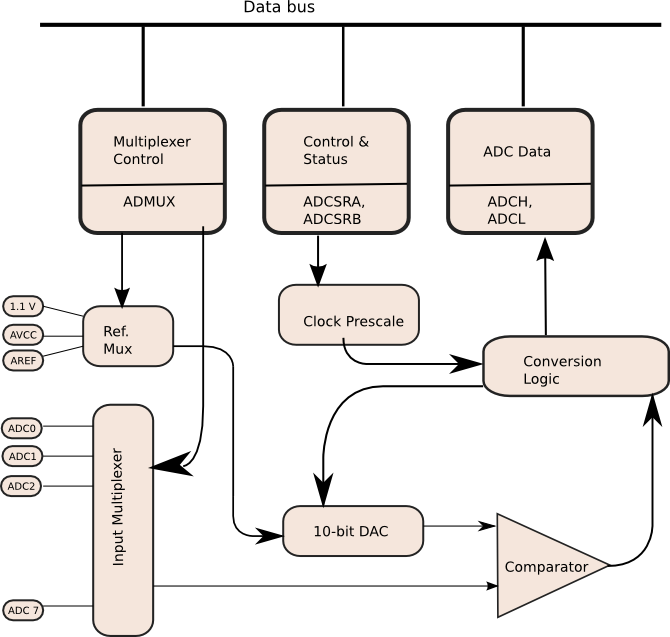
\includegraphics[width=\textwidth,keepaspectratio]{adc_blocks}
\caption{ADC block diagram}
\label{fig:ADC}
\end{figure}

ADC has multiplexer which help to select reference voltage for ADC. This reference voltage determines the range and resolution of the ADC. This leads to restriction in range of input voltage level.

As AVR has single 10 bit ADC so it can convert single analog channel at a time. But to convert multiple signal sources AVR microcontroller has multiplexer swithching circuit which swithches different analog signal channel at a time. 

ADC also need clock signal for its operation but it can't run at the full speed of the CPU. So clock to the ADC is prescaled which is kind of decreasing the clock frequency. This leads to challange for determining prescaler values. 

As ADC is a peripheral device, it needs start command called tigger to start the conversion process. AVR ADC can be triggered in two ways. One is through software triggering from code called Single Conversion mode. Another one is the auto triggering mode where the source of triggers are Timers, Interrupts and ADC itself. In auto triggering mode if ADC is self-triggered then it is said to be in free running mode.

\section{Registers for configuring ADC}
For using ADC certain registers must be configured for initialisation. These registers are used for selecting clock source, selecting channel and starting ADC conversion process.

\subsection{ADMUX}
\begin{figure}[h]
\centering
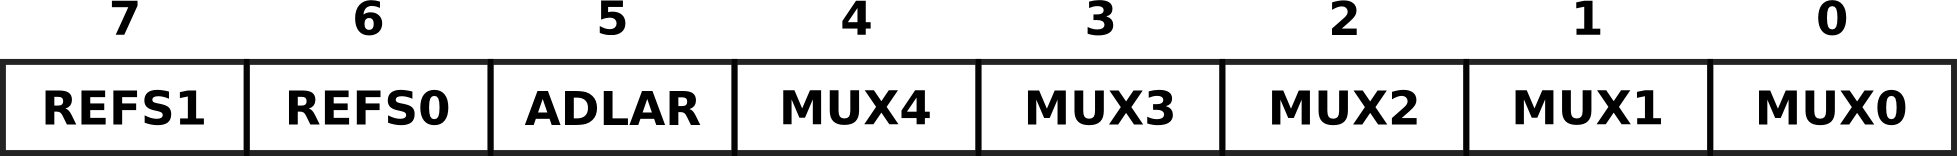
\includegraphics[width=\textwidth,keepaspectratio]{ADMUX}
\label{fig:ADMUX}
\end{figure}
\noindent
\textbf{REFSO, REFS1}- these bits are used for selecting the reference voltage for ADC. Table below shows various options.


\vspace{5mm}
\begin{tabular}{|c|c|c|}
\hline
\head{REFS0} & \head{REFS1} & \head{Voltage reference selection}\\
\hline
0 & 0 & AREF internal VREF turned off\\
0 & 1 & AVCC\\
1 & 0 & Reserved\\
1 & 1 & Internal 2.56 V \\
\hline
\end{tabular}
\vspace{5mm}

\noindent
\textbf{ADLAR}, if set left adjust the ADC value else right adjust the ADC value.

\noindent
\textbf{MUX4:0}, these bits together with MUX5 bit in ADCSRA register helps to select the one of the 16 channels.

\subsection{ADCSRA}
\begin{figure}[h]
\centering
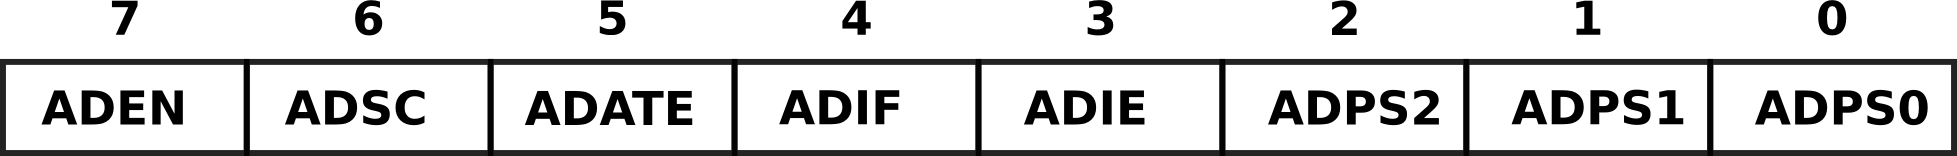
\includegraphics[width=\textwidth,keepaspectratio]{ADCSRA}
\label{fig:ADCSRA}
\end{figure}

\begin{description}
\item[ADEN] If set to one enables ADC
\item[ADSC] Set to one for starting the conversion
\item[ADATE] If set to one we can select trigger source for ADC 
\item[ADIF] This flag is set when conversion ends
\item[ADPS2:0] These bits are used for selecting the clock frequency for ADC
\end{description}

\vspace{5mm}
\begin{tabular}{|c|c|c|c|}
\hline
\head{ADPS2} & \head{ADPS1} & \head{ADPS0} & \head{Division factor}\\
\hline
0 & 0 & 0 & 2\\
0 & 0 & 1 & 2\\
0 & 1 & 0 & 4\\
0 & 1 & 1 & 8\\
1 & 0 & 0 & 16\\
1 & 0 & 1 & 32\\
1 & 1 & 0 & 64\\
1 & 1 & 1 & 128\\
\hline
\end{tabular}
\vspace{5mm}

\subsection{ADCSRB}
\begin{figure}[h]
\centering
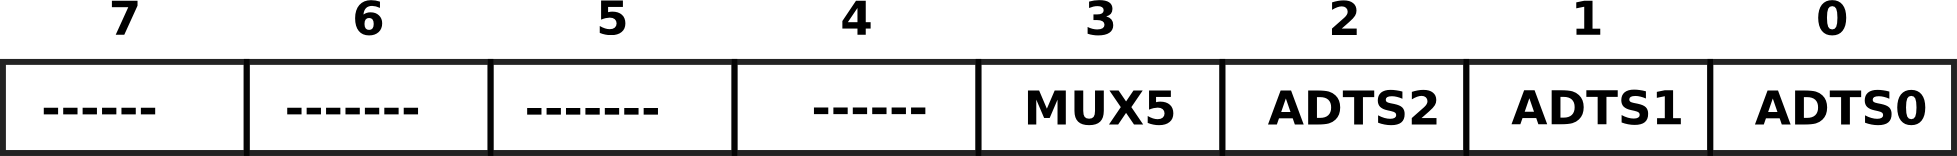
\includegraphics[width=\textwidth,keepaspectratio]{ADCSRB}
\label{fig:ADCSRB}
\end{figure}

\begin{description}
\item[MUX5] this bit together with ADMUX4:0 is used to select channel
\item[ADTS2:0] These bits are used for selecting the trigger source when ADATE is set in ADCSRA
\end{description}



\section{Minimum configuration of ADC}
For basic operation of the ADC we have to initialise following blocks in ADC peripheral block.
\begin{itemize}
\item Setting the prescaler for suitable clock source to ADC.
\item Selecting the required reference voltage.
\item Selecting the channel to sample
\item Selection of the trigger source for starting the conversion process.
\item Choosing 8 bit or 10 bit mode according the application requirements.
\end{itemize}

\section{First step to real world}
In this section, we will learn about various setting of the ADC for getting the sensor value and if value is less than certain limit sound the buzzer. For this project we will be running ADC in single conversion mode.
\subsection{Initalization of ADC}

For intialising the ADC first enable the ADC by setting the ADEN bit in ADCSRA. Then we have to select the frequency of clock source for ADC and reference voltage of ADC. For getting the accurate reading from the ADC, clock frequency to ADC block must be between 50 kHz to 200 kHz. So for this according to our CPU clock frequency 14745600 Hz, ADPS2=1, ADPS1=1 and ADPS0=1 will give clock frequency = FCPU/128 = 115.2 kHz. Finally select the AVCC=5V as the reference voltage by setting REFS1=0 and REFS1=0. So for initalisation values of ADMUX = 0x00 and ADCSRA = 0b10000111 = 0x87.
  

\begin{lstlisting}[language=C, caption=ADC initialization, escapechar=\~, frame=single]
//Function to Initialize ADC
void adc_init()
{
	ADMUX = 0x00;  //Vref=5V external 
	ADCSRA = 0x87; //ADEN=1 --- ADIE=1 --- ADPS2:0 = 1 1 1
}
\end{lstlisting}


\subsection{Reading the ADC value}
Now for reading the ADC value from real world we do the following steps:
\begin{itemize}
\item Select the channel of microcontroller where sensor is attached by setting MUX5:0 values.
For selecting the number one IR sensor in Firebird MUX4:0=0100 so 
\begin{lstlisting}[language=C, escapechar=\~, frame=single]
ADMUX| = 0x04.
\end{lstlisting}
\item Trigger the ADC by setting the start conversion bit,
\begin{lstlisting}[language=C, escapechar=\~, frame=single]
 ADCSRA| = 0x40.
\end{lstlisting}
\item Then poll the completion flag ADIF till the completion of conversion.
\begin{lstlisting}[language=C,escapechar=\~, frame=single]
	while((ADCSRA&0x10)==0);	//Wait for ADC conversion to complete
\end{lstlisting}

\item Then finally read the ADC value.
\end{itemize}

\begin{lstlisting}[language=C, caption=ADC initialization, escapechar=\~, frame=single]
//This Function accepts the Channel Number and returns the corresponding Analog Value 
unsigned char ADC_Conversion(unsigned char Ch)
{
	unsigned int adc_value;
	Ch = Ch & 0x07;  			
	ADMUX |= Ch;	   		
	ADCSRA = ADCSRA | 0x40;		//Set start conversion bit
	while((ADCSRA&0x10)==0);	//Wait for ADC conversion to complete
	adc_value=ADC;
	ADCSRA = ADCSRA|0x10; //clear ADIF (ADC Interrupt Flag) by writing 1 to it
	ADCSRB = 0x00;
	return adc_value;
}
\end{lstlisting}